\chapter{Results of competitive systems with different topologies}
\label{chapter:results}

In this chapter we present the results obtained through computational simulation of the minority games that include vicinity and are characterized by different network structures.

In Section \ref{sec:spacetime} we describe the role of information in competitive systems simulated with minority games in more detail, as it has already been mentioned in other parts of this work.
In Sections \ref{sec:fixed} and \ref{sec:hierarchical} we present the results for each network topology separately based on different parameters of the models.
After that in Section \ref{sec:confrontation} we confront different topologies to each other and explain the results.
Final two Sections, \ref{sec:spacetime2} and \ref{sec:final}, talk about the different role of information in the light of the results and conclude with some thoughts on competitive systems with limited resources. 

\section{Information in space and time}
\label{sec:spacetime}

From the initial studies of the competitive systems based on minority games we have seen that these models have two different phases of operation.
The separation of the two phases is defined by the relationship between the quantity of the information each agent can process and the number of agents, just as explained in subsection \ref{subsec:phasetransition} where $\alpha$ control parameter is defined.
The efficiency of the model, measured in the capacity to distribute the resources between agents, is best around the critical value of $\alpha$.
From this observation we can easily deduce that in order to optimize any kind of competitive system with similar mechanics we need to tinker with the $\alpha$ parameter to bring the volatility to its minimum.
Since $\alpha$ is defined as $\frac{2^M}{N}$ we are presented with a choice of either modifying the memory of the agents, their number, or both values at the same time.
Two important facts to note here and that have already been mentioned separately in previous chapters are: 
\begin{itemize}
\item In many systems to increase or decrease the number of agents involved is simply not realistic, as this could prove an inefficient and discriminatory politic. Think of a navigation system for vehicles or data packets. Should we remove or add more drivers/packets in order to optimize the system? Adding new elements to the model would only optimize the macroscopic behaviour of the system, while the performance of the initial agents present in model would not improve, it could actually worsen. On the other hand removing elements from the model would cause discrimination between who is allowed to participate and use the limited resource. Thus for the purpose of this thesis we have worked with a fixed number of agents inside our models and have focused on modifying the second parameter $M$, the memory of the agents
\item Even as we bring the volatility to its minimum through parameter modification it still remains a \textit{negative-sum-game}. The optimization consist in making the number of losing agents as low as possible, but it will always remain greater that the number of winning agents.
\end{itemize}

\begin{figure}[h]
\begin{center}
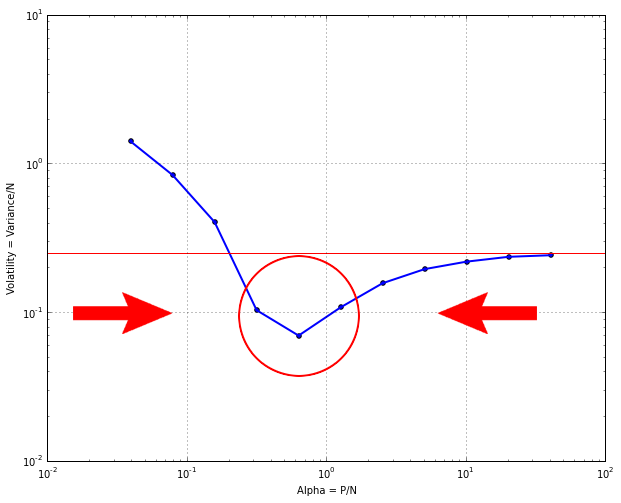
\includegraphics[scale=0.4]{images/results/alpha_to_norm_var2.png}
\caption{Plot of normalized variance versus control parameter $\alpha$ for a basic minority game}
\label{fig:normalized variance spacetime}
\end{center}
\end{figure}

We are left with tinkering with the quantity of information available to agents in order to minimize the volatility that is well defined and can be calculated with enough simulations from other parameters of the model, mainly the number of agents, but others like the number of strategies $S$ can influence it.
In Figure \ref{fig:normalized variance spacetime}, the example taken from subsection \ref{subsec:phasetransition}, we have pointed out the cases when the increase or the decrease of information is necessary.

Two more observations are needed before we dive into the analysis of the experimental results.
Foremost, not only can we optimize the system by changing the quantity of the information available to single agents, we can also work on the quality of that information. Of course the information added to the model has to be relevant to the system, but as we have seen from our results some scenarios are more desirable.
Let us assume $\mu(t) = (i_1,i_2,\ldots,i_m)$ the information available to the agent, represented as $m$ bits.
In classical minority games all the information is generated by the single global minority games, but nothing stops us from differentiating the information available.
Driven by the basic intuition that the differentiation of information is preferable and inspired by the fact that real world examples of the systems simulated offer the possibility to communicate, we have decided to optimize the model by adding the information from the community of the agent.
In this way we make a distinction between the global information based only on time, and the local community information based also on time but with a spatial component defined as the topology of the network.
This approach is realistically most probable, especially in the case when we have to increase the quantity of information, since temporally more distant data could not be available or due to the possible changing topology of the model (in real world agents participate for certain periods of time, until their needs are met) that renders temporally more distant data less reliable.
This intuition has brought us to include the locally available information and to test different network topologies described in \ref{chapter:vicinity}.

Second observation before diving into the experimental results is that when we have said that we only modify the brain size of agents and not the total number of agents, we have oversimplified our model.
Actually by adding local information and dividing the set of agents in communities, we are in a indirect way modifying the volatility of the model by creating smaller instances of minority games that bring the control parameter $\alpha$ closer to its critical value.
Of course the total number of agents remains the same and they are always present in the global minority game.

\section{Fixed community structures results}
\label{sec:fixed}

By fixed community structures we intend the fixed one-dimensional isolated communities described in Section \ref{sec:fixed communities}, sliding window one-dimensional communities defined in subsection \ref{subsec:sliding} and von Neumann neighbourhood described in Section \ref{sec:von neumann}.

In this section and the next one we use a new parameter $\beta$ to represent the relationship between the degree of each node to the number of total nodes, ie. the number of neighbouring agents versus the number of total agents.

\begin{displaymath}
\beta = \frac{d}{N}
\end{displaymath}

where $d$ is the mean degree of nodes in the network.

\subsection{Fixed one-dimensional communities}

The most simple topology is that of completely isolated local communities.
Also called patch neighbourhood it can be seen in \ref{fig:patch vicinity partial} that for various values of $\alpha$, different values of $\beta$ are optimal.
The data for the first two curves equivalent to models with information length $4$ and information length $6$ are shown in Tables \ref{table:fixed m4} and \ref{table:fixed m6}.
First three rows of each table has been highlighted and tells us what the minimum $\beta$ should be when planning a competitive system with certain $\alpha$ in order to minimize the loses.
So we can see that for $\alpha=0.03990025$ our best option is to keep our $\beta$ around $0.05$, that is divide the whole population in around 20 communities.
But $\alpha=0.03990025$ is still low to bring a system in a bit more efficient regime, so we look at the second curve from Figure \ref{fig:patch vicinity partial} where $\alpha=0.159601$.
For that value of $\alpha$ our best option is to keep our $\beta$ in the interval $[0.2,0.35]$, ie. divide the total number of agents in $3$ or $4$ big communities.

For successive network topologies we will only bring forth tables with best results, which here have been presented completely.

\begin{figure}[h!]
\begin{center}
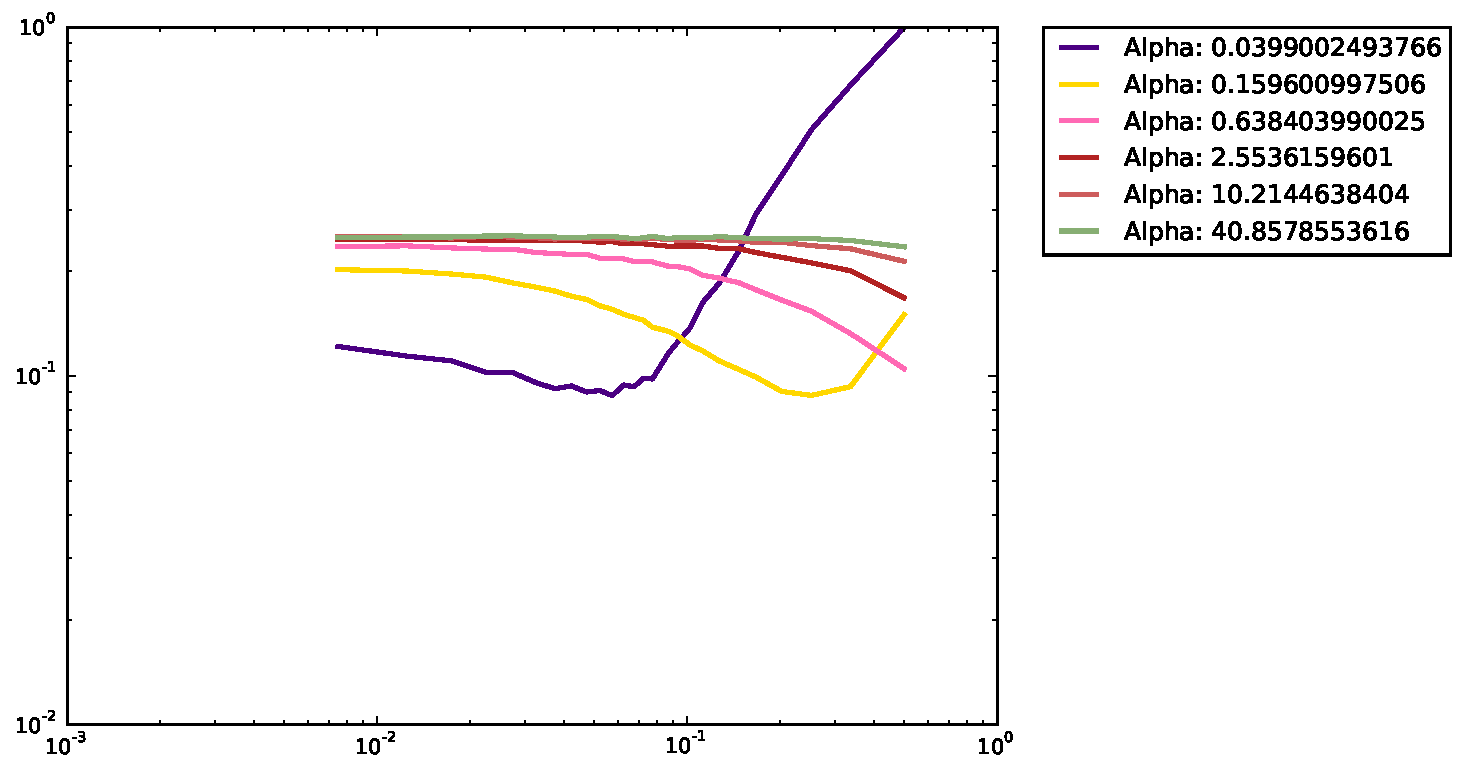
\includegraphics[scale=0.4]{images/results/vicinity_patch_n401_rounds10000_partial.pdf}
\caption{Plot of normalized variance versus control parameter $\beta$ for various values of $\alpha$  for fixed one-dimensional communities}
\label{fig:patch vicinity partial}
\end{center}
\end{figure}

\begin{table}
\tiny
\centering
\resizebox{\columnwidth}{!}{%
\begin{tabular}{lllllll}
\toprule
neighs &  M &    N &       alpha &         beta & meanNormVar &       var \\
\midrule
\rowcolor{Goldenrod}
    23 &  4 &  401 &  0.03990025 &   0.05735661 &  0.08778602 &  35.20219 \\
\rowcolor{Goldenrod}
    19 &  4 &  401 &  0.03990025 &   0.04738155 &   0.0899272 &  36.06081 \\
\rowcolor{Goldenrod}
    21 &  4 &  401 &  0.03990025 &   0.05236908 &  0.09083007 &  36.42286 \\
    15 &  4 &  401 &  0.03990025 &   0.03740648 &  0.09194704 &  36.87076 \\
    27 &  4 &  401 &  0.03990025 &   0.06733167 &  0.09309645 &  37.33168 \\
    17 &  4 &  401 &  0.03990025 &   0.04239401 &  0.09357988 &  37.52553 \\
    25 &  4 &  401 &  0.03990025 &   0.06234414 &   0.0941925 &  37.77119 \\
    13 &  4 &  401 &  0.03990025 &   0.03241895 &  0.09577665 &  38.40644 \\
    31 &  4 &  401 &  0.03990025 &   0.07730673 &  0.09799674 &  39.29669 \\
    29 &  4 &  401 &  0.03990025 &    0.0723192 &  0.09831647 &  39.42491 \\
    11 &  4 &  401 &  0.03990025 &   0.02743142 &   0.1021554 &  40.96432 \\
     9 &  4 &  401 &  0.03990025 &   0.02244389 &    0.102481 &  41.09487 \\
     7 &  4 &  401 &  0.03990025 &   0.01745636 &   0.1104009 &  44.27077 \\
     5 &  4 &  401 &  0.03990025 &   0.01246883 &   0.1139728 &  45.70309 \\
    35 &  4 &  401 &  0.03990025 &    0.0872818 &   0.1165516 &   46.7372 \\
     3 &  4 &  401 &  0.03990025 &  0.007481297 &   0.1214733 &   48.7108 \\
    37 &  4 &  401 &  0.03990025 &   0.09226933 &   0.1236184 &  49.57097 \\
    41 &  4 &  401 &  0.03990025 &    0.1022444 &   0.1373252 &  55.06739 \\
    45 &  4 &  401 &  0.03990025 &    0.1122195 &   0.1622121 &  65.04706 \\
    51 &  4 &  401 &  0.03990025 &     0.127182 &   0.1847199 &  74.07266 \\
    59 &  4 &  401 &  0.03990025 &    0.1471322 &   0.2288271 &  91.75965 \\
    67 &  4 &  401 &  0.03990025 &    0.1670823 &   0.2921831 &  117.1654 \\
    81 &  4 &  401 &  0.03990025 &     0.201995 &    0.375436 &  150.5499 \\
   101 &  4 &  401 &  0.03990025 &    0.2518703 &   0.5081641 &  203.7738 \\
   135 &  4 &  401 &  0.03990025 &    0.3366584 &   0.6818775 &  273.4329 \\
   201 &  4 &  401 &  0.03990025 &    0.5012469 &   0.9980141 &  400.2037 \\
\bottomrule
\end{tabular}%
}
\caption{Table of a model with $M=4$, with 2 bits dedicated to global game and 2 bits to local community information}
\label{table:fixed m4}
\end{table}

\begin{table}
\tiny
\centering
\resizebox{\columnwidth}{!}{%
\begin{tabular}{lllllll}
\toprule
neighs &  M &    N &     alpha &         beta & meanNormVar &       var \\
\midrule
\rowcolor{Goldenrod}
   101 &  6 &  401 &  0.159601 &    0.2518703 &  0.08792742 &  35.25889 \\
\rowcolor{Goldenrod}
    81 &  6 &  401 &  0.159601 &     0.201995 &  0.09028853 &   36.2057 \\
\rowcolor{Goldenrod}
   135 &  6 &  401 &  0.159601 &    0.3366584 &  0.09316642 &  37.35974 \\
    67 &  6 &  401 &  0.159601 &    0.1670823 &  0.09912482 &  39.74905 \\
    59 &  6 &  401 &  0.159601 &    0.1471322 &   0.1043162 &  41.83079 \\
    51 &  6 &  401 &  0.159601 &     0.127182 &   0.1103088 &  44.23381 \\
    45 &  6 &  401 &  0.159601 &    0.1122195 &   0.1179627 &  47.30303 \\
    41 &  6 &  401 &  0.159601 &    0.1022444 &   0.1226634 &  49.18803 \\
    37 &  6 &  401 &  0.159601 &   0.09226933 &    0.130943 &  52.50814 \\
    35 &  6 &  401 &  0.159601 &    0.0872818 &   0.1342167 &  53.82088 \\
    31 &  6 &  401 &  0.159601 &   0.07730673 &   0.1379274 &   55.3089 \\
    29 &  6 &  401 &  0.159601 &    0.0723192 &   0.1444711 &   57.9329 \\
    27 &  6 &  401 &  0.159601 &   0.06733167 &   0.1472001 &  59.02724 \\
   201 &  6 &  401 &  0.159601 &    0.5012469 &   0.1497855 &  60.06398 \\
    25 &  6 &  401 &  0.159601 &   0.06234414 &   0.1503266 &  60.28095 \\
    23 &  6 &  401 &  0.159601 &   0.05735661 &   0.1553099 &  62.27929 \\
    21 &  6 &  401 &  0.159601 &   0.05236908 &   0.1588146 &  63.68464 \\
    19 &  6 &  401 &  0.159601 &   0.04738155 &   0.1656952 &  66.44376 \\
    17 &  6 &  401 &  0.159601 &   0.04239401 &   0.1692265 &  67.85981 \\
    15 &  6 &  401 &  0.159601 &   0.03740648 &   0.1751308 &  70.22744 \\
    13 &  6 &  401 &  0.159601 &   0.03241895 &   0.1797978 &  72.09891 \\
    11 &  6 &  401 &  0.159601 &   0.02743142 &   0.1847625 &  74.08975 \\
     9 &  6 &  401 &  0.159601 &   0.02244389 &   0.1919552 &  76.97405 \\
     7 &  6 &  401 &  0.159601 &   0.01745636 &   0.1958953 &  78.55403 \\
     5 &  6 &  401 &  0.159601 &   0.01246883 &   0.1999117 &   80.1646 \\
     3 &  6 &  401 &  0.159601 &  0.007481297 &   0.2016834 &  80.87504 \\
\bottomrule
\end{tabular}%
}
\caption{Table of a model with $M=6$, with 3 bits dedicated to global game and 3 bits to local community information}
\label{table:fixed m6}
\end{table}

\subsection{Sliding window one-dimensional communities}

\begin{figure}[h]
\begin{center}
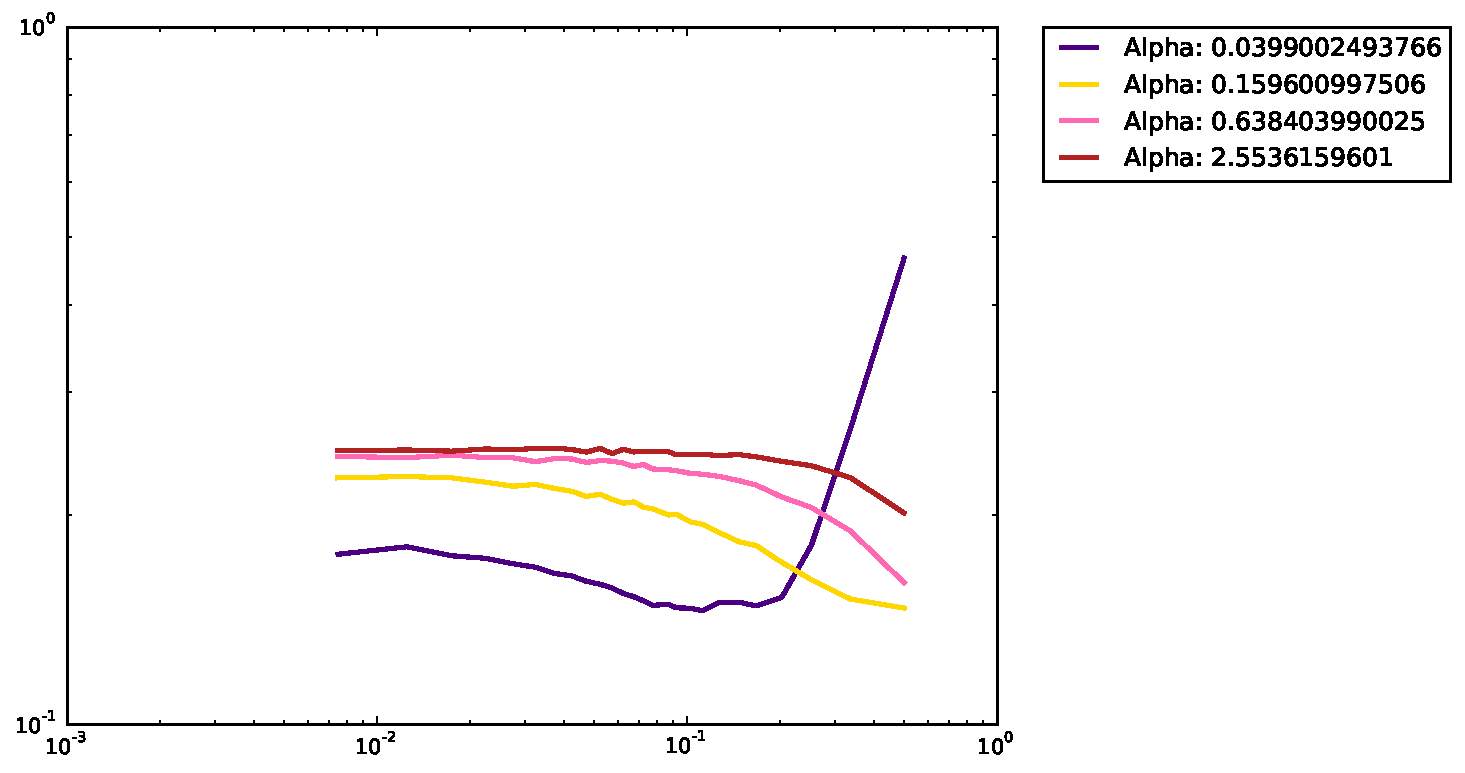
\includegraphics[scale=0.4]{images/results/vicinity_sliding_n401_rounds10000_partial.pdf}
\caption{Plot of normalized variance versus control parameter $\beta$ for various values of $\alpha$  for sliding window one-dimensional communities}
\label{fig:sliding vicinity partial}
\end{center}
\end{figure}

\subsection{Sliding window von Neumann neighbourhood}

\begin{figure}[h]
\begin{center}
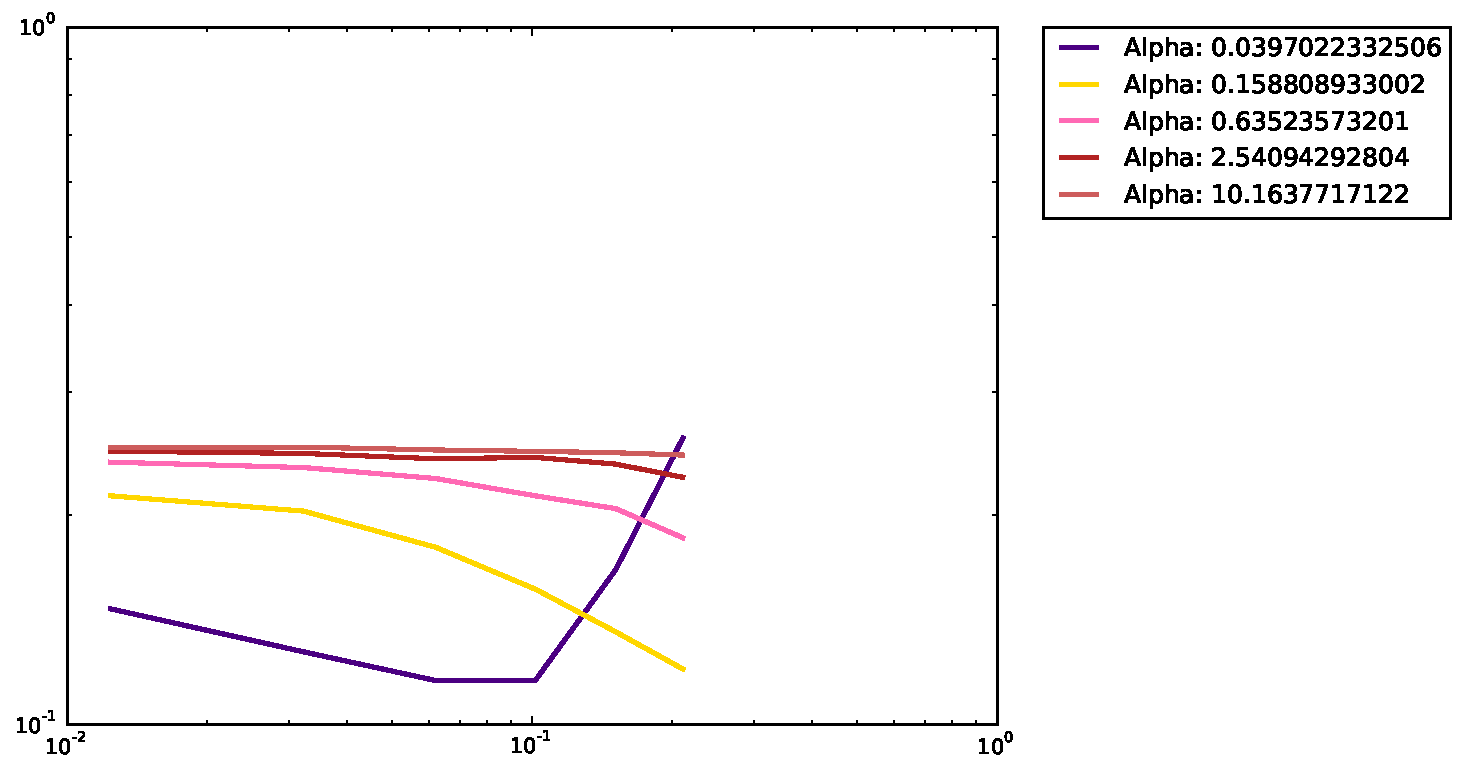
\includegraphics[scale=0.4]{images/results/vicinity_vonNeumann_n403_rounds10000_partial.pdf}
\caption{Plot of normalized variance versus control parameter $\beta$ for various values of $\alpha$  for sliding window two-dimensional communities with von Neumann vicinities}
\label{fig:von neumann vicinity partial}
\end{center}
\end{figure}


\section{Variable community structures results}
\label{sec:hierarchical}

\subsection{Scale free results}

\begin{figure}[h]
\begin{center}
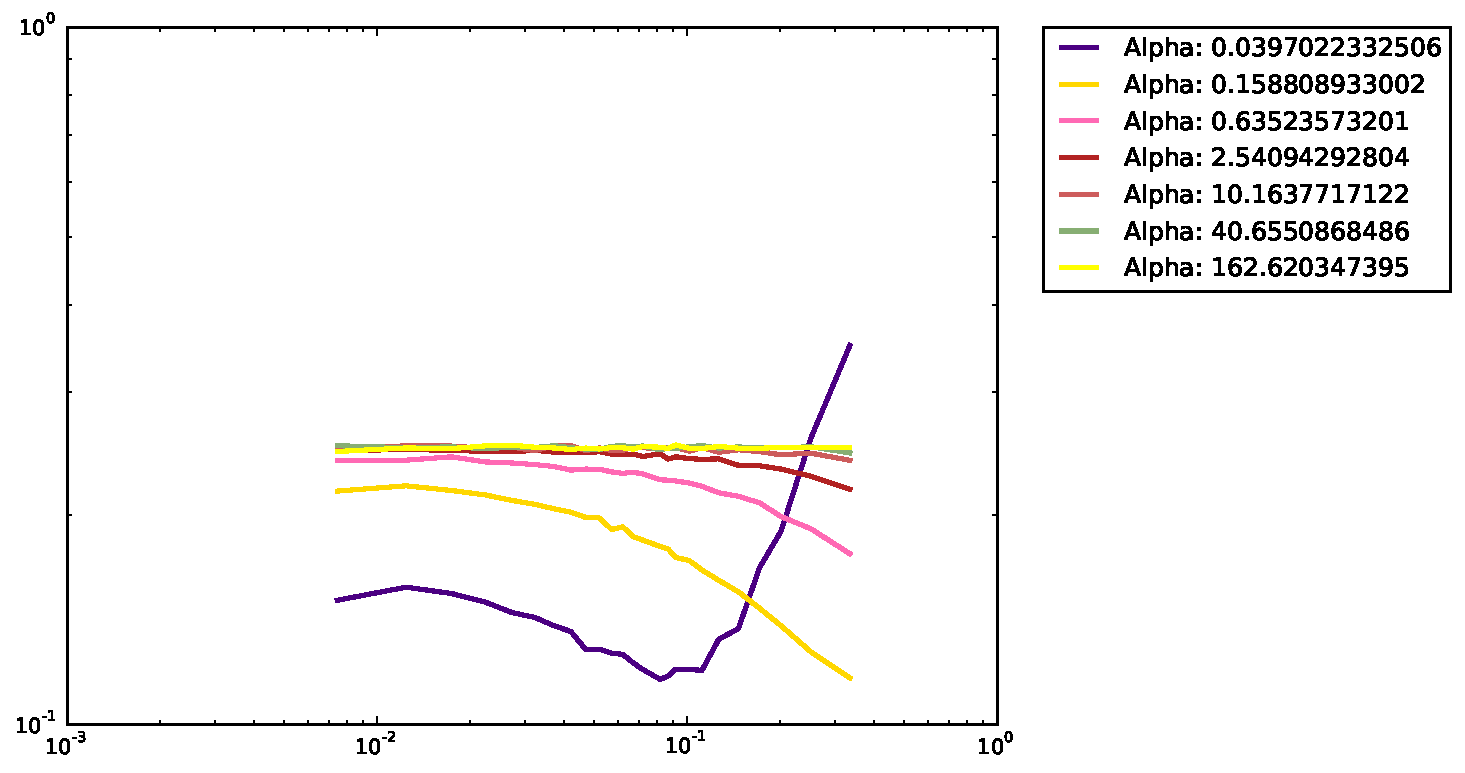
\includegraphics[scale=0.4]{images/results/vicinity_Barabasi_n403_rounds10000_partial.pdf}
\caption{Plot of normalized variance versus control parameter $\beta$ for various values of $\alpha$  for scale free communities generated with Barabasi-Albert algorithm}
\label{fig:scale free vicinity partial}
\end{center}
\end{figure}

\subsection{Small world results}

\begin{figure}[h]
\begin{center}
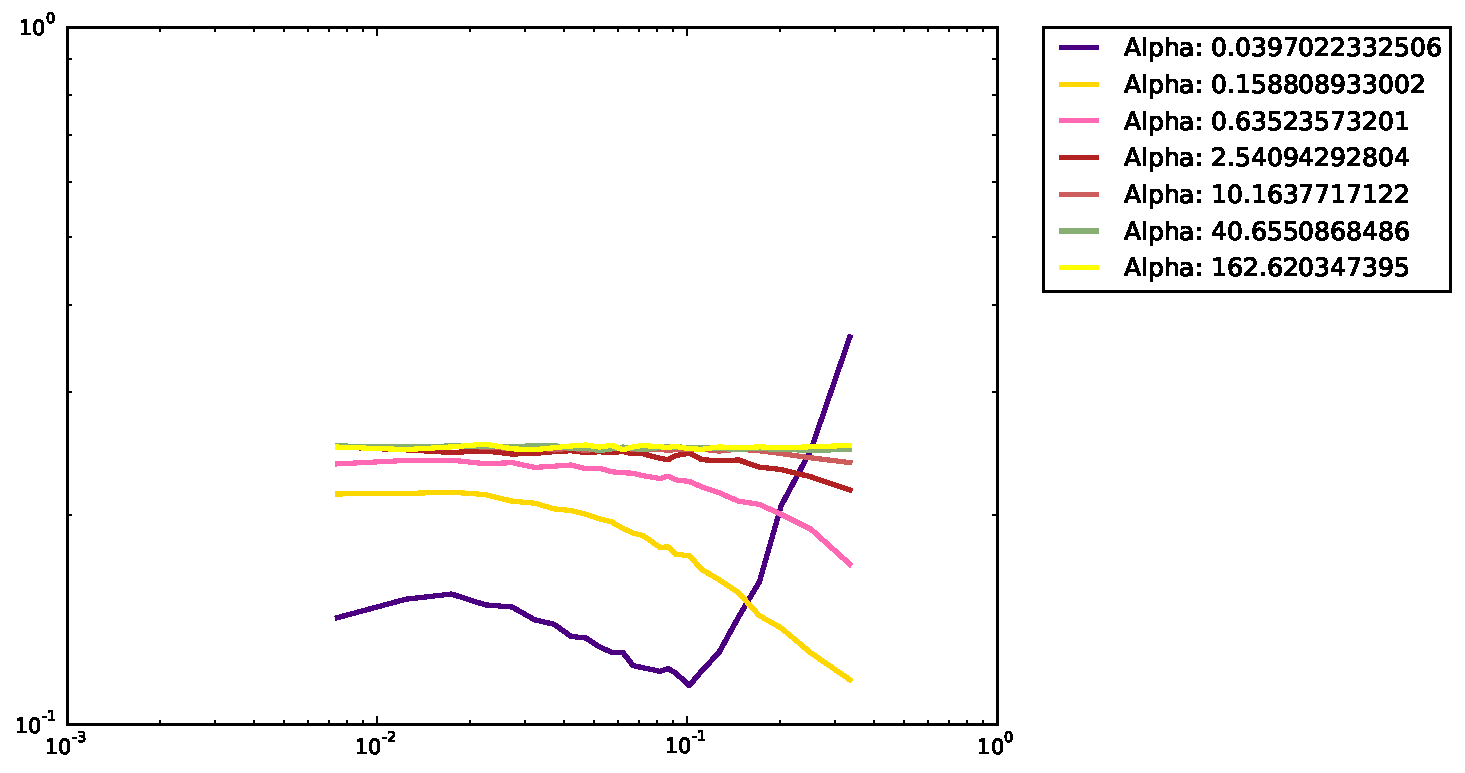
\includegraphics[scale=0.4]{images/results/vicinity_WattsStrogatz_n403_rounds10000_partial.pdf}
\caption{Plot of normalized variance versus control parameter $\beta$ for various values of $\alpha$  for small world communities generated with Watts-Strogatz algorithm}
\label{fig:scale free vicinity partial}
\end{center}
\end{figure}

\subsection{Hierarchical network results}

\section{Real world or artificial network}
\label{sec:confrontation}

\section{Information in space and time - second part}
\label{sec:spacetime2}

\section{Final considerations}
\label{sec:final}